% Architecture Description and system specifications
% 	* Multisensor IMS		
%		* Processing Stages
%		* Fusion approaches
%		* Methods and techniques
%		* Architecture proposal
%	* Validation approaches
%		* Transportation and Traffic Simulations
%			* Simulators Classification
%		* Intersection monitoring Datasets
%			* POSSi Dataset
%			* KoPER Dataset

\chapter [Architecture Description and System Specification]{Architecture Description and System Specification}
\chaptermark {System Description}

Although several types of sensors are used for intersection monitoring and supervision, the use of cameras, lasers and lidars has increased due to advances in sensors and computing capabilities. Such enhancements allows to deploy more of those types of sensors per scenario and it is required to define some processing stages from raw data capture through decision and control step. Also it is needed to test and validate the developments prior to a real and full functional implementation. The first part of this chapter describes the main stages in a intersection management system based on image and range sensors, and the methods used in these stages. Then an architecture proposal for the implementation of such a system is presented. Finally, two validation tools for IMS applications are described, simulation models and datasets.

\section{Multisensor IMS}

Multicamera and multilasers monitoring systems offer more information about environment that can be merged to provide a better representation of the whole scene, detect with more accuracy the objects in the intersection, and prevent possible incidents. For designing a single-sensor or multi-sensor IMS, there are some basic processing stages to have into account. In the case of a multisensor system, it is also required to analyse and determine which is the better fusion approach to use and in which of the processing stages this fusion should be performed, in order to get better results than a single-sensor based system.

\subsection{Processing Stages}

In the designing of an IMS, there are four main stages that have to be performed from the data source to final output: preprocessing, feature analysis, pattern recognition and situation assessment. The aim of the first stage is to extract data of interest from the raw sensor information, using filtering and background subtraction techniques to get the foreground of the scene, remove noise and irrelevant data. Spatio-temporal alignment of data is also performed in this stage. In the second stage, the objective is to identify elements within the foreground and extract relevant features of them. The third stage receives the set of features from the previous stage and performs recognition and classification tasks. Also, tracking and prediction of objects' state is performed based on historic information. In the fourth stage, object behaviour and inter-objects interaction are analysed to identify context and detect situation or events of interest. This output could be delivered to an optional fifth stage of decision and control, to a human operator, or to a traffic agent or institution, to take immediate actions on traffic control, issue traffic tickets, warn drivers about possible incidents or improve transportation policies in a long-term basis. In figure \ref{proc_stages}, previously described stages are depicted, and also is shown how the data volume is reduced while data meaning increases in the last stages.

\begin{figure}[ht!]
\centering
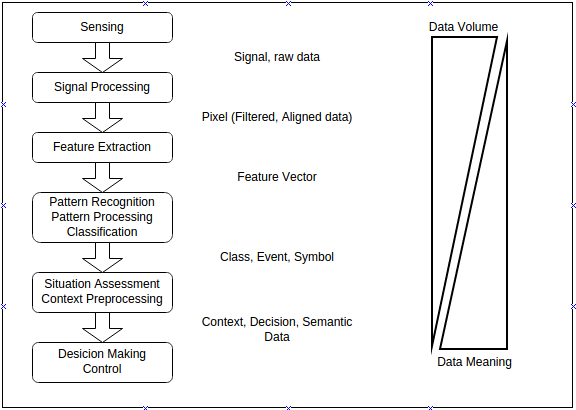
\includegraphics[scale=0.55]{fig/3/proc_stages.png}
\caption{Dataflow through processing stages in an IMS.}
\label{proc_stages}
\end{figure}


\subsection{Fusion approaches}

Depending on system design, if it has multiple sensors of the same type or different type, a data fusion approach should be chosen. When data came from same-type sensors, it is usually fused at low levels using techniques for temporal and/or spatial alignment, depending on sensors configuration. This is the case for a network of lasers or lidars or for multi-camera systems. If the system have different type of sensors, data from them may be fused at mid level, based on extracted features or classes on each subsystem; or may be fused at high level if each subsystem delivers control or decision outputs.

\section{Methods and techniques}

Different tasks could be performed in each aforementioned stages, as is referred in figure \ref{proc_stages_tasks}. Below there is a description of common concepts and methods associated with each of these tasks, some of them are sensor-independent and others are focused on a specific sensor or type of data. Additionally, these tasks could be used as fusion blocks for homogeneous or heterogeneous data.

\begin{figure}[ht!]
\centering
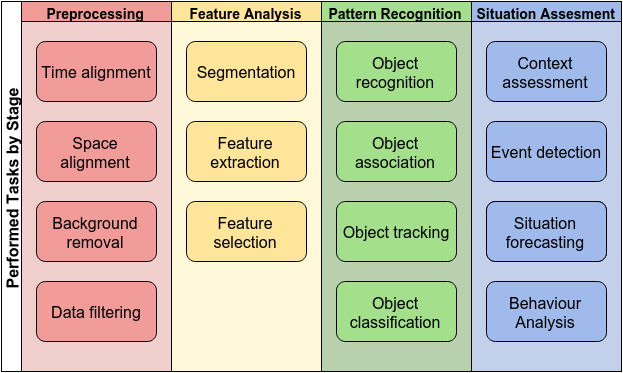
\includegraphics[scale=0.55]{fig/3/processing_stages_and_tasks.png}
\caption{Processing stages and tasks performed.}
\label{proc_stages_tasks}
\end{figure}

\subsection{Preprocessing}
\subsubsection{Background subtraction}
\subsubsection{Time-space alignment}
\subsection{Feature Analysis}
\subsubsection{Segmentation}
\subsubsection{Feature extraction}
\subsection{Pattern Recognition}
\subsubsection{Object association}
\subsubsection{Object tracking}
\subsubsection{Object classification}
\subsection{Situation Assessment}

\section{Validation approaches}

Before deploying an IMS, it is needed to test some of its components and validate their results. Two commonly used tools for this purpose are traffic simulation models and datasets, depending on the component to be tested. Below, a description of each one is presented.

\subsection{Transportation and Traffic Simulation}

A more detailed analysis of traffic simulation models and simulation platforms could be found in \cite{AdamsBoxill2000, Barcelo2000, Kitamura2005, Lieberman1992}
\subsubsection{Simulators Classification}
\subsection{Intersection monitoring Datasets}

As mentioned in section \ref{s23}, POSS-i and Ko-PER projects are leading the development of multisensor Intersection Management Systems. One of the contributions of these projects is the creation of datasets of such systems. They provide camera and laser information of a monitored intersection in Peking, China and Aschaffenburg, Germany, respectively. Next, a description of these two datasets will be given.

\subsubsection{POSSi Dataset }

POSSi dataset\footnote{Available at http://www.poss.pku.edu.cn/download.html}
\subsubsection{KoPER Dataset }

Ko-PER dataset\footnote{Available at http://www.uni-ulm.de/in/mrm/forschung/datensaetze.html}

The full description of this dataset is presented in \cite{Strigel2014}.

\section{Architecture proposal}